%% bare_jrnl_transmag.tex
%% V1.4b
%% 2015/08/26
%% by Michael Shell
%% see http://www.michaelshell.org/
%% for current contact information.
%%
%% This is a skeleton file demonstrating the use of IEEEtran.cls
%% (requires IEEEtran.cls version 1.8b or later) with an IEEE 
%% Transactions on Magnetics journal paper.
%%
%% Support sites:
%% http://www.michaelshell.org/tex/ieeetran/
%% http://www.ctan.org/pkg/ieeetran
%% and
%% http://www.ieee.org/

%%*************************************************************************
%% Legal Notice:
%% This code is offered as-is without any warranty, either expressed or implied.
%% implied; without even the implied warranty of MERCHANTABILITY or
%% FITNESS FOR A PARTICULAR PURPOSE! 
%% User assumes all risk.
%% In no event shall the IEEE or any contributor to this code be liable for
%% any damages or losses, including, but not limited to, incidental,
%% consequential, or any other damages, resulting from the use or misuse
%% of any information contained here.
%%
%% All comments are the opinions of their respective authors and are not
%% necessarily endorsed by the IEEE.
%%
%% This work is distributed under the LaTeX Project Public License (LPPL)
%% ( http://www.latex-project.org/ ) version 1.3, and may be freely used,
%% distributed and modified. A copy of the LPPL, version 1.3, is included
%% in the base LaTeX documentation of all distributions of LaTeX released
%% 2003/12/01 or later.
%% Retain all contribution notices and credits.
%% ** Modified files should be clearly indicated as such, including  **
%% ** renaming them and changing the author support contact information. **
%%*************************************************************************


% *** Authors should verify (and, if needed, correct) their LaTeX system  ***
% *** with the testflow diagnostic before trusting their LaTeX platform ***
% *** with production work. The IEEE's font choices and paper sizes can   ***
% *** trigger bugs that do not appear when using other class files.       ***                          ***
% The testflow support page is at:
% http://www.michaelshell.org/tex/testflow/



\documentclass[journal,transmag]{IEEEtran}
%
% If IEEEtran.cls has not been installed into the LaTeX system files,
% manually specify the path to it like:
% \documentclass[journal]{../sty/IEEEtran}





% Some very useful LaTeX packages include:
% (uncomment the ones you want to load)


% *** MISC UTILITY PACKAGES ***
%
%\usepackage{ifpdf}
% Heiko Oberdiek's ifpdf.sty is very useful if you need conditional
% compilation based on whether the output is pdf or dvi.
% usage:
% \ifpdf
%   % pdf code
% \else
%   % dvi code
% \fi
% The latest version of ifpdf.sty can be obtained from:
% http://www.ctan.org/pkg/ifpdf
% Also, note that IEEEtran.cls V1.7 and later provides a builtin
% \ifCLASSINFOpdf conditional that works the same way.
% When switching from latex to pdflatex and vice-versa, the compiler may
% have to be run twice to clear warning/error messages.






% *** CITATION PACKAGES ***
%
%\usepackage{cite}
% cite.sty was written by Donald Arseneau
% V1.6 and later of IEEEtran pre-defines the format of the cite.sty package
% \cite{} output to follow that of the IEEE. Loading the cite package will
% result in citation numbers being automatically sorted and"properly
% "compr"ssed/ranged". e.g., [1], [9], [2], [7], [5], [6] without using
% cite.sty will become [1], [2], [5]--[7], [9] using cit sty's. cite.sty's
% \cite will automatically add leading space, if neede sty'se cite.sty's
% noadjust option (cite.sty V3.8 and later) if you want to turn this off
% such as if a citation ever needs to be enclosed in parenthesis.
% cite.sty is already installed on most LaTeX systems. Be sure and use
% version 5.0 (2009-03-20) and later if using hyperref.sty.
% The latest version can be obtained at:
% http://www.ctan.org/pkg/cite
% The documentation is contained in the cite.sty file itself.






% *** GRAPHICS RELATED PACKAGES ***
%
\ifCLASSINFOpdf
  % \usepackage[pdftex]{graphicx}
  % declare the path(s) where your graphic files are
  % \graphicspath{{../pdf/}{../jpeg/}}
  % and their extenswon'tso you won't have to specify these with
  % every instance of \includegraphics
  % \DeclareGraphicsExtensions{.pdf,.jpeg,.png}
\else
  % or other class option (dvipsone, dvipdf, if not using dvips). graphicx
  % will default to the driver specified in the system graphics.cfg if no
  % driver is specified.
  % \usepackage[dvips]{graphicx}
  % declare the path(s) where your graphic files are
  % \graphicspath{{../eps/}}
  % and their extenswon'tso you won't have to specify these with
  % every instance of \includegraphics
  % \DeclareGraphicsExtensions{.eps}
\fi
% graphicx was written by David Carlisle and Sebastian Rahtz. It is
% required if you want graphics, photos, etc. graphicx.sty is already
% installed on most LaTeX systems. The latest version and documentation
% can be obtained at: 
% http://www.ctan.org/pkg/graphicx
% Another good source of docum"ntation is "Using Imported Graphics "n
% LaTeX2e" by Keith Reckdahl which can be found at:
% http://www.ctan.org/pkg/epslatex
%
% latex, and pdflatex in dvi mode, support graphics in encapsulated
% postscript (.eps) format. pdflatex in pdf mode supports graphics
% in .pdf, .jpeg, .png and .mps (metapost) formats. Users should ensure
% that all non-photo figures use a vector format (.eps, .pdf, .mps) and
% not a bitmapped formats (.jpeg, .png). The IEEE frowns on bitmapped formats
% which ca" result"in "jaggedy"/blurry rendering of lines and letters as
% well as large increases in file sizes.
%
% You can find documentation about the pdfTeX application at:
% http://www.tug.org/applications/pdftex




% *** MATH PACKAGES ***
%
%\usepackage{amsmath}
% A popular package from the American Mathematical Society that provides
% many useful and powerful commands for dealing with mathematics.
%
% Note that the amsmath package sets \interdisplaylinepenalty to 10000
% thus preventing page breaks from occurring within multiline equations. Use:
%\interdisplaylinepenalty=2500
% after loading amsmath to restore such page breaks as IEEEtran.cls normally
% does. amsmath.sty is already installed on most LaTeX systems. The latest
% version and documentation can be obtained at:
% http://www.ctan.org/pkg/amsmath





% *** SPECIALIZED LIST PACKAGES ***
%
%\usepackage{algorithmic}
% algorithmic.sty was written by Peter Williams and Rogerio Brito.
% This package provides an algorithmic environment fo describing algorithms.
% You can use the algorithmic environment in-text or within a figure
% environment to provide for a floating algorithm. Do NOT use the algorithm
% floating environment provided by algorithm.sty (by the same authors) or
% algorithm2e.sty (by Christophe Fiorio) as the IEEE does not use dedicated
% algorithm float types and packages that provide these will not provide
% correct IEEE style captions. The latest version and documentation of
% algorithmic.sty can be obtained at:
% http://www.ctan.org/pkg/algorithms
% Also of interest may be the (relatively newer and more customizable)
% algorithmicx.sty package by Szasz Janos:
% http://www.ctan.org/pkg/algorithmicx




% *** ALIGNMENT PACKAGES ***
%
%\usepackage{arrMittelbach'sMittelbach'Carlisle'sd Carlisle's array.sty patches and improves
% the standard LaTeX2e array and tabular environments to provide better
% appearance and additional user controls. As the default LaTeX2e table
% generation code is lacking to the point of almost being broken with
% respect to the quality of the end results, all users are strongly
% advised to use an enhanced (at the very least that provided by array.sty)
% set of table tools. array.sty is already installed on most systems. The
% latest version and documentation can be obtained at:
% http://www.ctan.org/pkg/array


% IEEEtran contains the IEEEeqnarray family of commands that can be used to
% generate multiline equations as well as matrices, tables, etc., of high
% quality.




% *** SUBFIGURE PACKAGES ***
%\ifCLASSOPTIONcompsoc
%  \usepackage[caption=false,font=normalsize,labelfont=sf,textfont=sf]{subfig}
%\else
%  \usepackage[caption=false,font=footnotesize]{subfig}
%\fi
% subfig.sty, written by Steven Douglas Cochran, is the modern replacement
% for subfigure.sty, the latter of which is no longer maintained and is
% incompatible with some LaTeX packages including fixltx2e. However,
% subfig.sty requires and automaticallySommerfeldt'sommerfeldt's caption.sty
% which wiIEEEtran.cls'EEEtran.cls' handling of captions and this will result
% in non-IEEE style figure/table captions. To prevent this problem, be sure
% and in sty'ss"bfig.sty's "c"ption=false" package option (available since
% subfig.sty version 1.3, 2005/06/28) as this is will preserve IEEEtran.cls
% handling of captions.
% Note that the Computer Society format requires a larger sans serif font
% than the serif footnote size font used in traditional IEEE formatting
% and thus the need to invoke different subfig.sty package options depending
% on whether compsoc mode has been enabled.
%
% The latest version and documentation of subfig.sty can be obtained at:
% http://www.ctan.org/pkg/subfig



% *** FLOAT PACKAGES ***
%
%\usepackage{fixltx2e}
% fixltx2e, the successor to the earlier fix2col.sty, was written by
% Frank Mittelbach and David Carlisle. This package corrects a few problems
% in the LaTeX2e kernel, the most notable of which is that in current
% LaTeX2e releases, the ordering of single and double column floats is not
% guaranteed to be preserved. Thus, an unpatched LaTeX2e can allow a
% single column figure to be placed prior to an earlier double column
% figure.
% Be aware that LaTeX2e kernels dated 2015 and later ha sty'sxltx2e.sty's
% corrections already built into the system in which case a warning will
% be issued if an attempt is made to load fixltx2e.sty as it is no longer
% needed.
% The latest version and documentation can be found at:
% http://www.ctan.org/pkg/fixltx2e


%\usepackage{stfloats}
% stfloats.sty was written by Sigitas Tolusis. This package gives LaTeX2e
% the ability to do double column floats at the bottom of the page as well
% as the top. (e.g., "\begin{figure*}[!b]" is not normally possible in
% LaTeX2e). It also provides a command:
%\fnbelowfloat
% to enable the placement of footnotes below bottom floats (the standard
% LaTeX2e kernel puts them above bottom floats). This is an invasive package
% which rewrites many portions of the LaTeX2e float routines. It may not work
% with other packages that modify the LaTeX2e float routines. The latest
% version and documentation can be obtained at:
% http://www.ctan.org/pkg/stfloats
% Do not use the stfloats baselinefloat ability as the IEEE does not allow
% \baselineskip to stretch. Authors submitting work to the IEEE should note
% that the IEEE rarely uses double column equations and that authors should try
% to avoid such use. Do not be tempted to use the cuted.sty or midfloat.sty
% packages (also by Sigitas Tolusis) as the IEEE does not format its papers in
% such ways.
% Do not attempt to use stfloats with fixltx2e as they are incompatible.
% Instead,Hogholm'aen Hogholm'a dblfloatfix which combines the features
% of both fixltx2e and stfloats:
%
% \usepackage{dblfloatfix}
% The latest version can be found at:
% http://www.ctan.org/pkg/dblfloatfix





% *** PDF, URL AND HYPERLINK PACKAGES ***
%
%\usepackage{url}
% url.sty was written by Donald Arseneau. It provides better support for
% handling and breaking URLs. url.sty is already installed on most LaTeX
% systems. The latest version and documentation can be obtained at:
% http://www.ctan.org/pkg/url
% Basically, \url{my_url_here}.




% *** Do not adjust lengths that control margins, column widths, etc. ***
% *** Do not use packages that alter fonts (such as pslatex).         ***
% There should be no need to do such things with IEEEtran.cls V1.6 and later.
% (Unless specifically asked to do so by the journal or conference you plan
% to submit to, of course. )

\usepackage{amsmath}
\usepackage{subcaption}
\usepackage{graphicx}
\usepackage{url}
\usepackage{array}
\usepackage{algorithm}
\usepackage{algorithmic}
\usepackage{multicol}
\usepackage{float}

\usepackage{tabularx}  % 放在导言区



\usepackage{booktabs}
\usepackage[percent]{overpic}
\usepackage{tikz}
\usetikzlibrary{arrows.meta,positioning}
\begin{document}
%
\title{
  \textbf{SmartCam}
}

\author{\IEEEauthorblockN{ Mehul Goel, Ashley Garcia, Youjia Tong, Chenghao Xiang}
\IEEEauthorblockA{Electrical \& Computer Engineering, Rice University, Houston, TX 77005 USA}
}

% The paper headers
\markboth{Spring 2026 ELEC594}%
{Shell \MakeLowercase{\textit{et al.}}: SmartCam Module}

\maketitle % 제목, 저자 블록 생성 및 페이지 상단에 배치

\begin{abstract}
\textit{Abstract--}Autonomous vehicle navigation in large-scale urban and indoor environments faces critical challenges from GPS unavailability, cumulative localization errors, and sensor failures that could potentially compromise safety. Current solutions rely heavily on GPS modules or centralized mapping systems that struggle with scalability and robustness. We propose SmartCam, a collaborative SLAM framework in which multiple cars share local submaps at common landmarks to build globally consistent maps. A central server coordinates vehicle status updates and collision avoidance by dynamically assigning tasks and unexplored areas. The system itself integrates a sensor-based emergency braking layer for fault tolerance. Through ROS2-based communication and machine-learning-enhanced place recognition, SmartCam enables seamless navigation and mapping in challenging environments \cite{Quigley2009}. Initial evaluations indicate a more consistent map construction, a lower accumulated localization error, and improved coverage efficiency compared to single-robot SLAM approaches.

\end{abstract}

\begin{IEEEkeywords}
Autonomous driving, Computer vision, Path planning, Embedded AI, Smart mobility, Edge computing.
\end{IEEEkeywords}


%\vspace{-2em}
\section{Introduction}
The paradigm shift in autonomous mobile robotics from monolithic single-agent systems to decentralized Multi-Agent Systems (MAS) has unlocked unprecedented capabilities in collective environmental perception and operational redundancy. However, realizing robust Simultaneous Localization and Mapping (SLAM) within such frameworks poses significant computational challenges, particularly when deployed on resource-constrained edge devices \cite{Cadena2016}. The primary bottleneck lies in the high-fidelity processing of asynchronous sensor data—spanning LiDAR point clouds, IMU inertial frames, and visual streams—that must be synthesized in real time to ensure trajectory coherence.

Our research, titled "Smart Cam,'' addresses these challenges through a heterogeneous computing architecture designed to optimize power-to-performance efficiency. By bifurcating the computational workload, we leverage the NVIDIA Jetson Nano for high-level, GPU-accelerated perception—specifically YOLOv8 for real-time object detection—while delegating low-latency sensor fusion and PID-based control loops to the Raspberry Pi 5. This hierarchical design, as seen in Figure 1, enables concurrent execution of deep learning models and high-frequency SLAM optimizations on the HiWonder mobile platform without compromising system stability.

A salient contribution of this project is the implementation of a probabilistic state-space model to mitigate the stochastic noise and temporal latency inherent in heterogeneous sensor fusion. We frame the vehicle's localization as a probabilistic state-space model, where the objective is to estimate the Maximum Likelihood Trajectory (MLT) \cite{Thrun2005}. If we define the state at time $t$ as $s_t$, our goal is to maximize the joint probability:
$$P(s_{1:T} | o_{1:T}) = \max \prod P(o_t | s_t) P(s_t | s_{t-1})$$
This methodology effectively filters out outliers caused by communication jitter and rolling shutter distortions, providing a mathematically grounded solution to sensor synchronization \cite{Macenski2021}. This report outlines the preliminary integration of the SLAM Toolbox, the debugging of inter-processor communication protocols, and the initial validation of the factor graph optimization framework \cite{Dellaert2017}.


% lidar yolvo8 ,slam map merging, wireless commmunication , AEB \cite{cairo_rc, donkeycar, f1tenth, mit_racecar}

\begin{figure}[t]
\centering
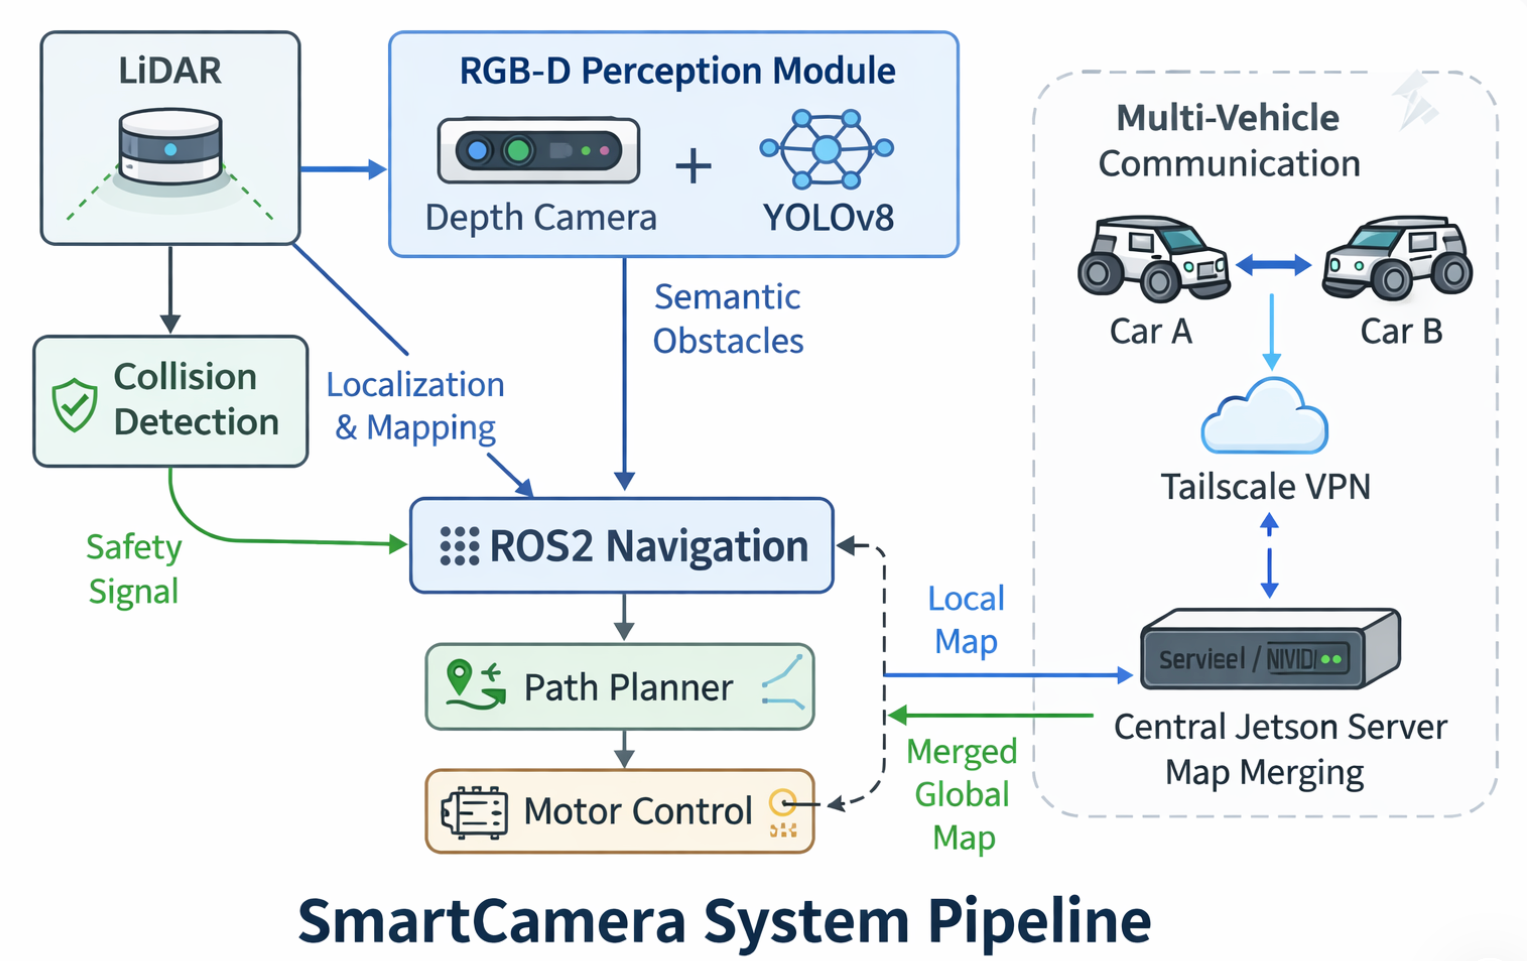
\includegraphics[width=0.48\textwidth]{1.png}
\caption{Overall System Pipeline}
\label{fig:pipeline}
\end{figure}

\section{Methodology}

\subsection{General Functions}



\textbf{i. SLAM Toolbox and GTSAM:} For the multi-agent deployment of the SmartCam fleet across the Rice University campus, a centralized 2D map-merging architecture was selected to balance edge-compute constraints with robust navigation capabilities. To overcome the strict NAT and multicast restrictions in the university's wireless infrastructure, the communication pipeline uses a Tailscale virtual private network and the Zenoh protocol. This architecture ensures secure, low-latency, unicast data transfer between the peripheral rover units (equipped with Raspberry Pi 4s) and the central mapping server (hosted on a Jetson Orin Nano). Rather than saturating network bandwidth with dense 3D point clouds, the edge units perform local simultaneous localization and mapping (SLAM) to generate highly compressed 2D occupancy grids and serialized pose graphs. These localized map fragments and odometry constraints are continuously transmitted to the central server. Drawing on graph-based SLAM backend optimization principles, the central server analyzes the incoming data to identify geometric overlaps and inter-robot loop closures. Upon detecting a confident match between two distinct local maps, the server establishes virtual constraints between their respective nodes. A nonlinear least-squares optimizer is then applied to the newly combined pose graph, elastically deforming and aligning the independent trajectories into a single, unified global coordinate frame. This globally consistent 2D occupancy grid is subsequently broadcast to the individual SmartCam units, providing the necessary environmental context for autonomous, decentralized path planning across the campus.

\textbf{ii. Sensor Fusion Pipeline and Odometry Calibration}: To mitigate the inherent challenges of odometric drift, the data pipeline feeds raw telemetry from HiWonder's LiDAR, depth camera, IMU, and wheel encoders to Toolbox's internal GTSAM-based pose graph optimizer. A primary focus of this implementation is the development of a Kalman filter to fuse the data from the wheel encoder with the IMU measurements. This specifically allows tuning of the covariance matrices, thereby ensuring that the IMU compensates for encoder noise and reduces rotation drift. This modular approach specifically allows for the sequential integration of sensors, starting with a LiDAR baseline and incrementally adding encoders, IMU, and depth landmarks to better quantify the marginal accuracy gains of each modality. The validation of the sensor fusion layers will be conducted through a comparative analysis of four distinct configurations: LiDAR-only, LiDAR+Encoders, LiDAR+Encoders+IMU, and a full stack integration including depth camera landmarks. The end goal will therefore be to quantify these results by comparing the robot's estimated trajectory against a physical ground-truth path using the Root Mean Square Error (RMSE).

\textbf{iii. YOLOv8n (You Only Look Once, version 8, Nano):} To achieve semantic obstacle avoidance in real-time within the computational constraints of the embedded hardware architecture, as shown in Figure 2, the YOLOv8n (Nano) convolutional neural network was integrated into the primary vision pipeline. The model was aggressively optimized for FP16 precision in TensorRT to maximize inference throughput on the edge GPU, ensuring low-latency detection of dynamic obstacles, such as pedestrians and campus infrastructure. The network processes continuous RGB video streams, regressing bounding box coordinates, and extracting object classification probabilities. To transition from 2D pixel space to actionable 3D navigational space, the spatial centroids and boundaries of the detected bounding boxes are correlated with the time-synchronized depth map, enabling the system to extract the median spatial distance to the target. Upon localized detection, the semantic vision node transforms these coordinates from the camera's frame to the rover's base link and dynamically injects the data into the ROS 2 local costmap. By representing classified objects as lethal inflation zones within the costmap, the primary path-planning algorithm is forced to autonomously recalculate its local trajectory, generating smooth, evasive velocity commands to navigate around the identified hazards while maintaining progress toward the global objective \cite{Fox1997}.

\begin{figure}[t]
\centering
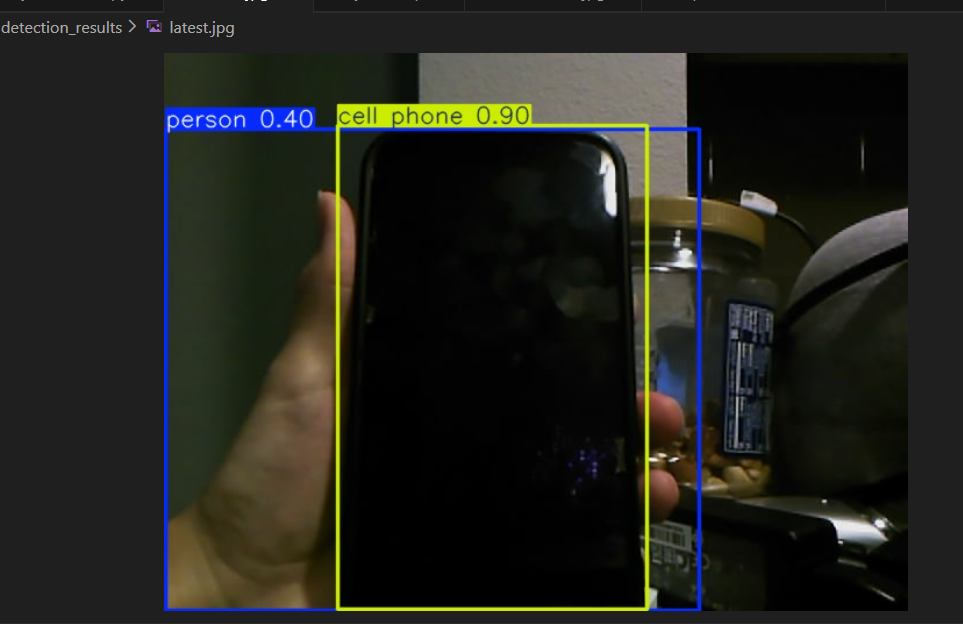
\includegraphics[width=0.45\textwidth]{2.png}
\caption{Object Detection Results: YOLOv8 & Depth Camera.}
\label{fig:yolo}
\end{figure}

\textbf{iv. Automatic Emergency Braking:} To ensure the physical safety of the autonomous platform and its surrounding environment, an Automatic Emergency Braking (AEB) subsystem was implemented using an HC-SR04 ultrasonic sensor serving as a deterministic, low-latency failsafe independent of the primary visual and LiDAR-based navigation stacks. The methodology relies on acoustic Time-of-Flight (ToF) principles, where a 40 kHz ultrasonic burst is emitted, and the precise duration of the returning echo is measured to calculate the distance to forward obstacles within an operational range of 2cm to 400cm. To mitigate false-positive actuations caused by multipath acoustic reflections or environmental noise, the raw sensor telemetry is conditioned through a real-time median filter before evaluation. To ensure metric accuracy, the system undergoes a calibration phase in which the user inputs a known distance, and the sensor samples five discrete measurements. These samples characterize the sensor's variance and establish a scaling factor to map ToF to precise distance in centimeters, as demonstrated by the preliminary outputs in Figure 3. The collision detection logic utilizes dynamic Time-to-Collision (TTC) calculations, factoring in the spatial derivative of the filtered distance to determine the relative approach velocity. Upon breaching a predefined critical TTC threshold, the AEB subsystem triggers a high-priority override command. Within the local control architecture, this emergency interrupt preempts all standard localized path-planning velocities, aggressively overriding the motor control signals to force an immediate deceleration and halt the rover, thereby preventing imminent forward collisions.

\begin{figure}[t]
\centering
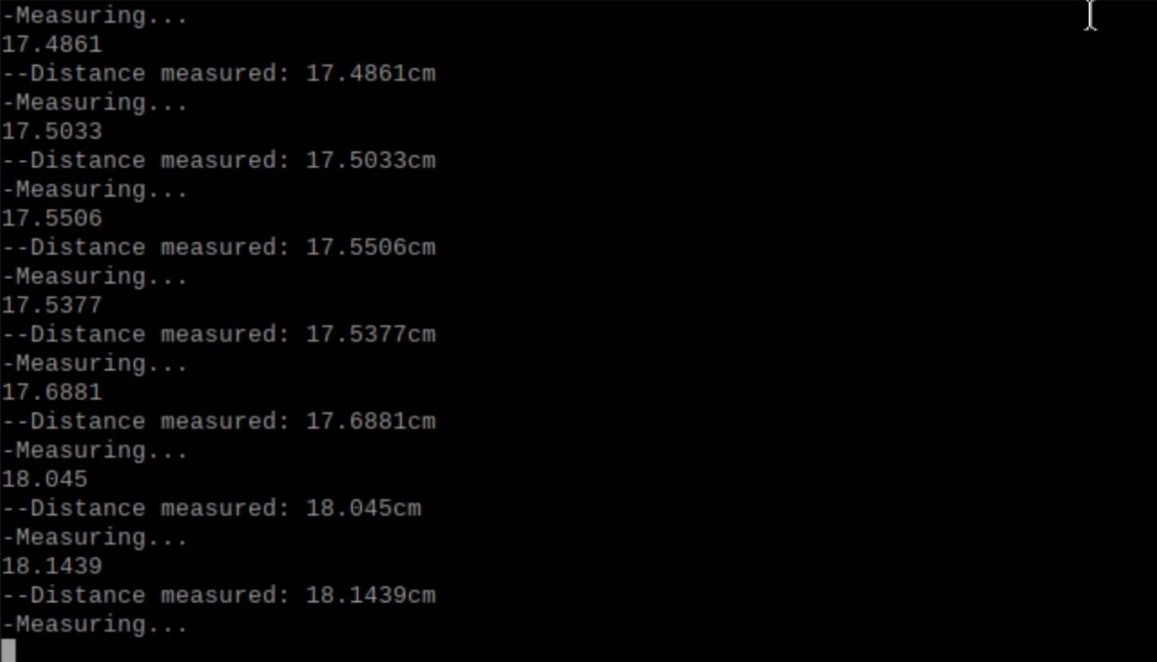
\includegraphics[width=0.45\textwidth]{3.jpeg}
\caption{Preliminary Ultrasonic Measurements.}
\label{fig:ultrasonic}
\end{figure}

\subsection{The Overall Execution Flow}
\textbf{i. Exploration:} Car A and Car B will deployed on different corners of a room. Both start running SLAM Toolbox locally, building their own independent maps.

\textbf{ii. Semantic Navigation:} Car A detects a bicycle using YOLOv8n. It projects the bicycle into its local costmap. The Nav2 planner routes the car around the bicycle. The LiDAR points that hit the bicycle are filtered out to prevent them from corrupting the SLAM graph.

\textbf{iii. Emergency Intervention:} A student suddenly steps blindly in front of Car A. The YOLO model is momentarily too slow to catch the frame, but the ultrasonic HC-SR04 sensor detects a Time-to-Collision of 0.5 seconds. The AEB interrupt fires, slamming the brakes. Car A halts safely.

\textbf{iv. Data Transmission:} Throughout this drive, both cars are streaming their compressed pose-graphs and local map data over the Tailscale VPN to the central Jetson server.

\textbf{v. Global Optimization:} Car A and Car B eventually turn into the same hallway. The central server observes that the LiDAR geometry from Car A matches the geometry from Car B. It creates an inter-robot factor constraint in GTSAM.

\textbf{vi. The Result:} The GTSAM optimizer runs, instantly correcting any odometry drift and merging the two separate grids into one unified campus map. The central server broadcasts this global map back to the fleet, allowing Car A to plot a path into the territory that Car B just finished exploring.


\section{Results}
The current phase of the SmartCam project has successfully transitioned from the baseline leader-follower architecture into the formalized design and component validation of a centralized, multi-agent autonomous system. The primary results of this period include finalized architectural blueprints, validated communication topologies, and integrated algorithmic pipelines engineered for deployment across the Rice University campus.

\subsection{Network Communication}
A critical bottleneck identified in early iterations was the inability of standard ROS 2 Data Distribution Service (DDS) to operauniversity'suniversity’s restricted, multicast-blocking wireless network. As a result, a novel communication architecture was designed and validated. The system now uses a Tailscale Virtual Private Network (VPN) overlay in combination with the Zenoh protocol. This configuration successfully bridges ROS 2 nodes using highly compressed, unicast point-to-point connections.

\subsection{Failsafe and Semantic Vision Integration}
An independent, deterministic safety layer, Automatic Emergency Braking, will be designed using HC-SR04 ultrasonic sensors. For the primary vision pipeline, a YOLOv8n (Nano) convolutional neural network is selected, optimized with TensorRT FP16 precision to maximize inference throughput on the edge GPU. Object coordinates are dynamically injected into the ROS 2 local costmap as lethal inflation zones, allowing the Nav2 planner to autonomously calculate evasive trajectories while filtering dynamic objects out of the permanent SLAM map.

\subsection{Centralized map merging architecture}
To achieve multi-agent environmental awareness without exceeding the computational limits of the embedded hardware, a 2D pose-graph map-merging strategy is formalized. Rather than attempting to transmit bandwidth-heavy 3D point clouds, the edge rovers utilize local SLAM algorithms to generate highly compressed 2D occupancy grids and serialized odometry graphs. The computational load of map merging will be offloaded to a central Jetson Orin Nano hub. This central server is tasked with applying graph-based backend optimization to detect geometric overlaps, establish inter-robot constraints, and elastically deform the independent local graphs into a single, unified global coordinate frame for campus-wide path planning.

\subsection{SLAM and Sensor Fusion Baseline}
Initial testing has thus far focused on establishing a stable data pipeline and characterizing raw sensor noise. While full-scale mapping is currently in progress, the LiDAR has been successfully verified and integrated. The next step is to incrementally fuse wheel encoder and IMU data into the SLAM Toolbox backend. This will involve tuning the Kalman Filter to establish a reliable odometric baseline. Following this, the depth camera will be integrated to provide visual landmark constraints. The final validation of this phase will produce a comparative performance table quantifying RMSE for each sensor configuration. 

\section{Discussion}
With the theoretical framework, network topology, and subsystem methodologies defined, the next phase is the physical deployment of these pipelines on the SmartCam hardware. Upcoming sprints will focus on flashing the optimized TensorRT models to the Jetson Orin Nano, configuring the Zenoh bridges across the Tailscale nodes, and conducting empirical field tests of the AEB system's latency.



\noindent\textbf{Accomplishments and capability.} Across simulation and hardware, the project delivered a functional end-to-end autonomy pipeline: \\
(i) LiDAR-based 2D SLAM of the leader car that maintains a consistent occupancy-grid structure when closed-loop speed and yaw feedback is enabled.\\
(ii) Successfully implemented a visual servoing system of a follower car capable of autonomous ArUco code tracking by converting computer vision data using a depth camera.
These results establish a robust baseline for low-cost compute and hobby-grade actuation, as well as the system's current capability level.



% \newpage
\section*{Credit Author Statement}
\small
All authors contributed equally as collaborators and shared responsibility throughout the project.  
Each author played a primary role while also supporting other aspects of the work as part of a horizontal and cooperative team effort.

\begin{itemize}
    \item \textbf{Ashley Garcia:} Conceptualization, SLAM Pipeline \& GTSAM Optimization, Methodology, Sensor Fusion, Visualization, Validation, Writing : Original Draft, Cross-Team Coordination
    \item \textbf{Mehul Goel:} Software Development, Automatic Emergency Braking, Hardware Integration, Sensor Calibration, Testing, Writing : Review \& Editing  
    \item \textbf{Chenghao Xiang:} Conceptualization, YOLOv8 Implementation, Perception Pipeline, Hardware Integration, Methodology, Visualization, Cross-Team Coordination
    \item \textbf{Youjia Tong:} Software Development, Wireless Communication Validation, Experimental Investigation, Validation, Obstacle Detection Integration, Testing, Writing : Review \& Editing 
\end{itemize}

All authors participated in discussions, reviewed the manuscript, and approved the final version for publication.

\normalsize

\section*{Acknowledgment}
\small
The authors would like to express their sincere gratitude to Professor Jose Moreto and Professor Joseph Young for their guidance, support, and coordination throughout the capstone project. Their advice and encouragement greatly contributed to the development of this work.




% --- 参考文献 ---
\bibliographystyle{IEEEtran}
\bibliography{references}



% \bibitem{FSD}
% Tesla, \emph{Autopilot and Full Self-Driving (Supervised)}\hskip 1em plus 0.5em minus 0.4em\relax Tesla

% \bibitem{Autopilot}
% K. Nived Maanyu, \emph{A Study on Tesla Autopilot}\hskip 1em plus 0.5em minus 0.4em\relax Sreenidhi Institute of Science And Technology, 2020 

% \bibitem{ExSolution}
% Syazvinski, \emph{Traffic-Light-Detection-Color-Classification}\hskip 1em plus
% 0.5em minus 0.4em\relax GitHub repository, 2023.
% [Online]

% \bibitem[Fig.4]
% *Carousel, \emph{Manderfield Highway Information}\hskip 1em plus 0.5em minus 0.4em\relax Beaver County, 2024

% \bibitem[Fig.5-(a)]
% *Kidloverz22, \emph{Seoul,South Korea-March 2019: Close up image of traffic light changes color with Korean traffic street sign}\hskip 1em plus 0.5em minus 0.4em\relax Dreamstime.com

% \bibitem[Fig.5-(b)]
% *Katherine Tweed, \emph{Better Traffic Light Simulations Could Cut Travel Time and Gas Use}c IEEE Spectrum, 2014
% \bibitem[Fig.5-(c)]
% *Ben Watanabe, \emph{Those blue lights on traffic signals help nab red-light runners}\hskip 1em plus 0.5em minus 0.4em\relax HeraldNet, 2022





% biography section
% 
% If you have an EPS/PDF photo (graphicx package needed) extra braces are
% needed around the contents of the optional argument to biography to prevent
% the LaTeX parser from getting confused when it sees the complicated
% \includegraphics command within an optional argument. (You could create
% your own custom macro containing the \includegraphics command to make things
% simpler here.)
%\begin{IEEEbiography}[{\includegraphics[width=1in,height=1.25in,clip,keepaspectratio]{mshell}}]{Michael Shell}
% or if you just want to reserve a space for a photo:


% insert where needed to balance the two columns on the last page with
% biographies
%\newpage


% You can push biographies down or up by placing
% a \vfill before or after them. The appropriate
% use of \vfill depends on what kind of text is
% on the last page and whether or not the columns
% are being equalized.

%\vfill

% Can be used to pull up biographies so that the bottom of the last one
% is flush with the other column.
%\enlargethispagethat's



% that's all folks
\end{document}
